\hypertarget{group__nfsft}{
\section{NFSFT - Nonequispaced fast spherical Fourier transform}
\label{group__nfsft}\index{NFSFT - Nonequispaced fast spherical Fourier transform@{NFSFT - Nonequispaced fast spherical Fourier transform}}
}
\subsection*{Data Structures}
\begin{CompactItemize}
\item 
struct \hyperlink{structnfsft__plan}{nfsft\_\-plan}
\begin{CompactList}\small\item\em Structure for a NFSFT transform plan. \item\end{CompactList}\item 
struct \hyperlink{structnfsft__wisdom}{nfsft\_\-wisdom}
\begin{CompactList}\small\item\em Wisdom structure. \item\end{CompactList}\end{CompactItemize}
\subsection*{Defines}
\begin{CompactItemize}
\item 
\#define \hyperlink{group__nfsft_ga25}{NFSFT\_\-NORMALIZED}~(1U $<$$<$ 0)
\begin{CompactList}\small\item\em By default, all computations are performed with respect to the unnormalized basis functions \[ \tilde{Y}_k^n(\vartheta,\varphi) = P_k^{|n|}(\cos\vartheta) \mathrm{e}^{\mathrm{i} n \varphi}. \] If this flag is set, all computations are carried out using the $L_2$- normalized basis functions \[ Y_k^n(\vartheta,\varphi) = \sqrt{\frac{2k+1}{4\pi}} P_k^{|n|}(\cos\vartheta) \mathrm{e}^{\mathrm{i} n \varphi}. \]. \item\end{CompactList}\item 
\#define \hyperlink{group__nfsft_ga26}{NFSFT\_\-USE\_\-NDFT}~(1U $<$$<$ 1)
\begin{CompactList}\small\item\em If this flag is set, the fast NFSFT algorithms (see \hyperlink{group__nfsft_ga8}{nfsft\_\-trafo}, \hyperlink{group__nfsft_ga9}{nfsft\_\-adjoint}) will use internally the exact but usually slower direct NDFT algorithm in favor of fast but approximative NFFT algorithm. \item\end{CompactList}\item 
\#define \hyperlink{group__nfsft_ga27}{NFSFT\_\-USE\_\-DPT}~(1U $<$$<$ 2)
\begin{CompactList}\small\item\em If this flag is set, the fast NFSFT algorithms (see \hyperlink{group__nfsft_ga8}{nfsft\_\-trafo}, \hyperlink{group__nfsft_ga9}{nfsft\_\-adjoint}) will use internally the usually slower direct DPT algorithm in favor of the fast FPT algorithm. \item\end{CompactList}\item 
\#define \hyperlink{group__nfsft_ga28}{NFSFT\_\-MALLOC\_\-X}~(1U $<$$<$ 3)
\begin{CompactList}\small\item\em If this flag is set, the init methods (see \hyperlink{group__nfsft_ga1}{nfsft\_\-init} , \hyperlink{group__nfsft_ga2}{nfsft\_\-init\_\-advanced} , and \hyperlink{group__nfsft_ga3}{nfsft\_\-init\_\-guru}) will allocate memory and the method \hyperlink{group__nfsft_ga10}{nfsft\_\-finalize} will free the array {\tt x} for you. \item\end{CompactList}\item 
\#define \hyperlink{group__nfsft_ga29}{NFSFT\_\-MALLOC\_\-F\_\-HAT}~(1U $<$$<$ 5)
\begin{CompactList}\small\item\em If this flag is set, the init methods (see \hyperlink{group__nfsft_ga1}{nfsft\_\-init} , \hyperlink{group__nfsft_ga2}{nfsft\_\-init\_\-advanced} , and \hyperlink{group__nfsft_ga3}{nfsft\_\-init\_\-guru}) will allocate memory and the method \hyperlink{group__nfsft_ga10}{nfsft\_\-finalize} will free the array {\tt f\_\-hat} for you. \item\end{CompactList}\item 
\#define \hyperlink{group__nfsft_ga30}{NFSFT\_\-MALLOC\_\-F}~(1U $<$$<$ 6)
\begin{CompactList}\small\item\em If this flag is set, the init methods (see \hyperlink{group__nfsft_ga1}{nfsft\_\-init} , \hyperlink{group__nfsft_ga2}{nfsft\_\-init\_\-advanced} , and \hyperlink{group__nfsft_ga3}{nfsft\_\-init\_\-guru}) will allocate memory and the method \hyperlink{group__nfsft_ga10}{nfsft\_\-finalize} will free the array {\tt f} for you. \item\end{CompactList}\item 
\#define \hyperlink{group__nfsft_ga31}{NFSFT\_\-PRESERVE\_\-F\_\-HAT}~(1U $<$$<$ 7)
\begin{CompactList}\small\item\em If this flag is set, it is guaranteed that during an execution of \hyperlink{group__nfsft_ga6}{ndsft\_\-trafo} or \hyperlink{group__nfsft_ga8}{nfsft\_\-trafo} the content of {\tt f\_\-hat} remains unchanged. \item\end{CompactList}\item 
\#define \hyperlink{group__nfsft_ga32}{NFSFT\_\-PRESERVE\_\-X}~(1U $<$$<$ 8)
\begin{CompactList}\small\item\em If this flag is set, it is guaranteed that during an execution of \hyperlink{group__nfsft_ga6}{ndsft\_\-trafo}, \hyperlink{group__nfsft_ga8}{nfsft\_\-trafo} or \hyperlink{group__nfsft_ga7}{ndsft\_\-adjoint}, \hyperlink{group__nfsft_ga9}{nfsft\_\-adjoint} the content of {\tt x} remains unchanged. \item\end{CompactList}\item 
\#define \hyperlink{group__nfsft_ga33}{NFSFT\_\-PRESERVE\_\-F}~(1U $<$$<$ 9)
\begin{CompactList}\small\item\em If this flag is set, it is guaranteed that during an execution of \hyperlink{group__nfsft_ga7}{ndsft\_\-adjoint} or \hyperlink{group__nfsft_ga9}{nfsft\_\-adjoint} the content of {\tt f} remains unchanged. \item\end{CompactList}\item 
\#define \hyperlink{group__nfsft_ga34}{NFSFT\_\-DESTROY\_\-F\_\-HAT}~(1U $<$$<$ 10)
\begin{CompactList}\small\item\em If this flag is set, it is explicitely allowed that during an execution of \hyperlink{group__nfsft_ga6}{ndsft\_\-trafo} or \hyperlink{group__nfsft_ga8}{nfsft\_\-trafo} the content of {\tt f\_\-hat} may be changed. \item\end{CompactList}\item 
\#define \hyperlink{group__nfsft_ga35}{NFSFT\_\-DESTROY\_\-X}~(1U $<$$<$ 11)
\begin{CompactList}\small\item\em If this flag is set, it is explicitely allowed that during an execution of \hyperlink{group__nfsft_ga6}{ndsft\_\-trafo}, \hyperlink{group__nfsft_ga8}{nfsft\_\-trafo} or \hyperlink{group__nfsft_ga7}{ndsft\_\-adjoint}, \hyperlink{group__nfsft_ga9}{nfsft\_\-adjoint} the content of {\tt x} may be changed. \item\end{CompactList}\item 
\#define \hyperlink{group__nfsft_ga36}{NFSFT\_\-DESTROY\_\-F}~(1U $<$$<$ 12)
\begin{CompactList}\small\item\em If this flag is set, it is explicitely allowed that during an execution of \hyperlink{group__nfsft_ga7}{ndsft\_\-adjoint} or \hyperlink{group__nfsft_ga9}{nfsft\_\-adjoint} the content of {\tt f} may be changed. \item\end{CompactList}\item 
\#define \hyperlink{group__nfsft_ga37}{NFSFT\_\-NO\_\-DIRECT\_\-ALGORITHM}~(1U $<$$<$ 13)
\begin{CompactList}\small\item\em If this flag is set, the transforms \hyperlink{group__nfsft_ga6}{ndsft\_\-trafo} and \hyperlink{group__nfsft_ga7}{ndsft\_\-adjoint} do not work. \item\end{CompactList}\item 
\#define \hyperlink{group__nfsft_ga38}{NFSFT\_\-NO\_\-FAST\_\-ALGORITHM}~(1U $<$$<$ 14)
\begin{CompactList}\small\item\em If this flag is set, the transforms \hyperlink{group__nfsft_ga8}{nfsft\_\-trafo} and \hyperlink{group__nfsft_ga9}{nfsft\_\-adjoint} do not work. \item\end{CompactList}\item 
\#define \hyperlink{group__nfsft_ga39}{NFSFT\_\-ZERO\_\-F\_\-HAT}~(1U $<$$<$ 16)
\begin{CompactList}\small\item\em If this flag is set, the transforms \hyperlink{group__nfsft_ga9}{nfsft\_\-adjoint} and \hyperlink{group__nfsft_ga7}{ndsft\_\-adjoint} set all unused entries in {\tt f\_\-hat} not corresponding to spherical Fourier coefficients to zero. \item\end{CompactList}\item 
\hypertarget{group__nfsft_ga40}{
\#define \hyperlink{group__nfsft_ga40}{NFSFT\_\-INDEX}(k, n, plan)~((2$\ast$(plan) $\rightarrow$ N+2)$\ast$((plan) $\rightarrow$ N-n+1)+(plan) $\rightarrow$ N+k+1)}
\label{group__nfsft_ga40}

\begin{CompactList}\small\item\em This helper macro expands to the index $i$ corresponding to the spherical Fourier coefficient $f_hat(k,n)$ for $0 \le k \le N$, $-k \le n \le k$ with \[ (N+2)(N-n+1)+N+k+1 \]. \item\end{CompactList}\item 
\hypertarget{group__nfsft_ga41}{
\#define \hyperlink{group__nfsft_ga41}{NFSFT\_\-F\_\-HAT\_\-SIZE}(N)~((2$\ast$N+2)$\ast$(2$\ast$N+2))}
\label{group__nfsft_ga41}

\begin{CompactList}\small\item\em This helper macro expands to the logical size of a spherical Fourier coefficients array for a bandwidth N. \item\end{CompactList}\item 
\hypertarget{group__nfsft_ga42}{
\#define {\bf BWEXP\_\-MAX}~10}
\label{group__nfsft_ga42}

\item 
\hypertarget{group__nfsft_ga43}{
\#define {\bf BW\_\-MAX}~1024}
\label{group__nfsft_ga43}

\item 
\hypertarget{group__nfsft_ga44}{
\#define {\bf ROW}(k)~(k$\ast$(wisdom.N\_\-MAX+2))}
\label{group__nfsft_ga44}

\item 
\hypertarget{group__nfsft_ga45}{
\#define {\bf ROWK}(k)~(k$\ast$(wisdom.N\_\-MAX+2)+k)}
\label{group__nfsft_ga45}

\item 
\#define \hyperlink{group__nfsft_ga46}{NFSFT\_\-DEFAULT\_\-NFFT\_\-CUTOFF}~6
\begin{CompactList}\small\item\em The default NFFT cutoff parameter. \item\end{CompactList}\item 
\#define \hyperlink{group__nfsft_ga47}{NFSFT\_\-DEFAULT\_\-THRESHOLD}~1000
\begin{CompactList}\small\item\em The default threshold for the FPT. \item\end{CompactList}\item 
\#define \hyperlink{group__nfsft_ga48}{NFSFT\_\-BREAK\_\-EVEN}~5
\begin{CompactList}\small\item\em The break-even bandwidth $N \in \mathbb{N}_0$. \item\end{CompactList}\end{CompactItemize}
\subsection*{Enumerations}
\begin{CompactItemize}
\item 
enum {\bf bool} \{ {\bf false} =  0, 
{\bf true} =  1
 \}
\end{CompactItemize}
\subsection*{Functions}
\begin{CompactItemize}
\item 
void \hyperlink{group__nfsft_ga1}{nfsft\_\-init} (\hyperlink{structnfsft__plan}{nfsft\_\-plan} $\ast$plan, int N, int M)
\begin{CompactList}\small\item\em Creates a transform plan. \item\end{CompactList}\item 
void \hyperlink{group__nfsft_ga2}{nfsft\_\-init\_\-advanced} (\hyperlink{structnfsft__plan}{nfsft\_\-plan} $\ast$plan, int N, int M, unsigned int nfsft\_\-flags)
\begin{CompactList}\small\item\em Creates a transform plan. \item\end{CompactList}\item 
void \hyperlink{group__nfsft_ga3}{nfsft\_\-init\_\-guru} (\hyperlink{structnfsft__plan}{nfsft\_\-plan} $\ast$plan, int N, int M, unsigned int nfsft\_\-flags, int nfft\_\-flags, int nfft\_\-cutoff)
\begin{CompactList}\small\item\em Creates a transform plan. \item\end{CompactList}\item 
void \hyperlink{group__nfsft_ga4}{nfsft\_\-precompute} (int N, double kappa, unsigned int nfsft\_\-flags, unsigned int fpt\_\-flags)
\begin{CompactList}\small\item\em Performes precomputation up to the next power of two with respect to a given bandwidth $N \in \mathbb{N}_2$. \item\end{CompactList}\item 
void \hyperlink{group__nfsft_ga5}{nfsft\_\-forget} ()
\begin{CompactList}\small\item\em Forgets all precomputed data. \item\end{CompactList}\item 
void \hyperlink{group__nfsft_ga6}{ndsft\_\-trafo} (\hyperlink{structnfsft__plan}{nfsft\_\-plan} $\ast$plan)
\begin{CompactList}\small\item\em Executes a direct NDSFT, i.e. \item\end{CompactList}\item 
void \hyperlink{group__nfsft_ga7}{ndsft\_\-adjoint} (\hyperlink{structnfsft__plan}{nfsft\_\-plan} $\ast$plan)
\begin{CompactList}\small\item\em Executes a direct adjoint NDSFT, i.e. \item\end{CompactList}\item 
void \hyperlink{group__nfsft_ga8}{nfsft\_\-trafo} (\hyperlink{structnfsft__plan}{nfsft\_\-plan} $\ast$plan)
\begin{CompactList}\small\item\em Executes a NFSFT, i.e. \item\end{CompactList}\item 
void \hyperlink{group__nfsft_ga9}{nfsft\_\-adjoint} (\hyperlink{structnfsft__plan}{nfsft\_\-plan} $\ast$plan)
\begin{CompactList}\small\item\em Executes an adjoint NFSFT, i.e. \item\end{CompactList}\item 
void \hyperlink{group__nfsft_ga10}{nfsft\_\-finalize} (\hyperlink{structnfsft__plan}{nfsft\_\-plan} $\ast$plan)
\begin{CompactList}\small\item\em Destroys a plan. \item\end{CompactList}\item 
\hypertarget{group__nfsft_ga11}{
void {\bf nfsft\_\-precompute\_\-x} (\hyperlink{structnfsft__plan}{nfsft\_\-plan} $\ast$plan)}
\label{group__nfsft_ga11}

\item 
double \hyperlink{group__nfsft_ga12}{alpha\_\-al} (int k, int n)
\begin{CompactList}\small\item\em Computes three-term recurrence coefficients $\alpha_k^n$ of associated Legendre functions. \item\end{CompactList}\item 
double \hyperlink{group__nfsft_ga13}{beta\_\-al} (int k, int n)
\begin{CompactList}\small\item\em Computes three-term recurrence coefficients $\beta_k^n$ of associated Legendre functions. \item\end{CompactList}\item 
double \hyperlink{group__nfsft_ga14}{gamma\_\-al} (int k, int n)
\begin{CompactList}\small\item\em Computes three-term recurrence coefficients $\gamma_k^n$ of associated Legendre functions. \item\end{CompactList}\item 
\hypertarget{group__nfsft_ga15}{
void {\bf alpha\_\-al\_\-row} (double $\ast$alpha, int N, int n)}
\label{group__nfsft_ga15}

\item 
\hypertarget{group__nfsft_ga16}{
void {\bf beta\_\-al\_\-row} (double $\ast$beta, int N, int n)}
\label{group__nfsft_ga16}

\item 
\hypertarget{group__nfsft_ga17}{
void {\bf gamma\_\-al\_\-row} (double $\ast$gamma, int N, int n)}
\label{group__nfsft_ga17}

\item 
void \hyperlink{group__nfsft_ga18}{alpha\_\-al\_\-all} (double $\ast$alpha, int N)
\begin{CompactList}\small\item\em Compute three-term-recurrence coefficients $\alpha_{k-1}^n$ of associated Legendre functions for $k,n = 0,1,\ldots,N$. \item\end{CompactList}\item 
void \hyperlink{group__nfsft_ga19}{beta\_\-al\_\-all} (double $\ast$alpha, int N)
\begin{CompactList}\small\item\em Compute three-term-recurrence coefficients $\beta_{k-1}^n$ of associated Legendre functions for $k,n = 0,1,\ldots,N$. \item\end{CompactList}\item 
void \hyperlink{group__nfsft_ga20}{gamma\_\-al\_\-all} (double $\ast$alpha, int N)
\begin{CompactList}\small\item\em Compute three-term-recurrence coefficients $\gamma_{k-1}^n$ of associated Legendre functions for $k,n = 0,1,\ldots,N$. \item\end{CompactList}\item 
void \hyperlink{group__nfsft_ga21}{eval\_\-al} (double $\ast$x, double $\ast$y, int size, int k, double $\ast$alpha, double $\ast$beta, double $\ast$gamma)
\begin{CompactList}\small\item\em Evaluates an associated Legendre polynomials $P_k^n(x,c)$ using the Clenshaw-algorithm. \item\end{CompactList}\item 
int \hyperlink{group__nfsft_ga22}{eval\_\-al\_\-thresh} (double $\ast$x, double $\ast$y, int size, int k, double $\ast$alpha, double $\ast$beta, double $\ast$gamma, double threshold)
\begin{CompactList}\small\item\em Evaluates an associated Legendre polynomials $P_k^n(x,c)$ using the Clenshaw-algorithm if it no exceeds a given threshold. \item\end{CompactList}\item 
void \hyperlink{group__nfsft_ga23}{c2e} (\hyperlink{structnfsft__plan}{nfsft\_\-plan} $\ast$plan)
\begin{CompactList}\small\item\em Converts coefficients $\left(b_k^n\right)_{k=0}^M$ with $M \in \mathbb{N}_0$, $-M \le n \le M$ from a linear combination of Chebyshev polynomials \[ f(\cos\vartheta) = \sum_{k=0}^{2\lfloor\frac{M}{2}\rfloor} a_k (\sin\vartheta)^{n\;\mathrm{mod}\;2} T_k(\cos\vartheta) \] to coefficients $\left(c_k^n\right)_{k=0}^M$ matching the representation by complex exponentials \[ f(\cos\vartheta) = \sum_{k=-M}^{M} c_k \mathrm{e}^{\mathrm{i}k\vartheta} \] for each order $n=-M,\ldots,M$. \item\end{CompactList}\item 
void \hyperlink{group__nfsft_ga24}{c2e\_\-transposed} (\hyperlink{structnfsft__plan}{nfsft\_\-plan} $\ast$plan)
\begin{CompactList}\small\item\em Transposed version of the function \hyperlink{group__nfsft_ga23}{c2e}. \item\end{CompactList}\end{CompactItemize}
\subsection*{Variables}
\begin{CompactItemize}
\item 
static struct \hyperlink{structnfsft__wisdom}{nfsft\_\-wisdom} \hyperlink{group__nfsft_ga0}{wisdom} = \{false,0U\}
\begin{CompactList}\small\item\em The global wisdom structure for precomputed data. \item\end{CompactList}\end{CompactItemize}


\subsection{Detailed Description}
This module implements nonuniform fast spherical Fourier transforms. In the following, we abbreviate the term \char`\"{}nonuniform fast spherical Fourier transform\char`\"{} by NFSFT.\hypertarget{group__nfsft_Preliminaries}{}\subsection{Preliminaries}\label{group__nfsft_Preliminaries}
This section summarises basic definitions and properties related to spherical Fourier transforms.\hypertarget{group__nfsft_sc}{}\subsubsection{Spherical Coordinates}\label{group__nfsft_sc}
Every point in $\mathbb{R}^3$ can be described in {\em spherical\/} {\em coordinates\/} by a vector $(r,\vartheta,\varphi)^{\mathrm{T}}$ with the radius $r \in \mathbb{R}^{+}$ and two angles $\vartheta \in [0,\pi]$, $\varphi \in [-\pi,\pi)$. We denote by $\mathbb{S}^2$ the two-dimensional unit sphere embedded into $\mathbb{R}^3$, i.e. \[ \mathbb{S}^2 := \left\{\mathbf{x} \in \mathbb{R}^{3}:\; \|\mathbf{x}\|_2=1\right\} \] and identify a point from $\mathbb{S}^2$ with the corresponding vector $(\vartheta,\varphi)^{\mathrm{T}}$. The spherical coordinate system is illustrated in the following figure:  \mbox{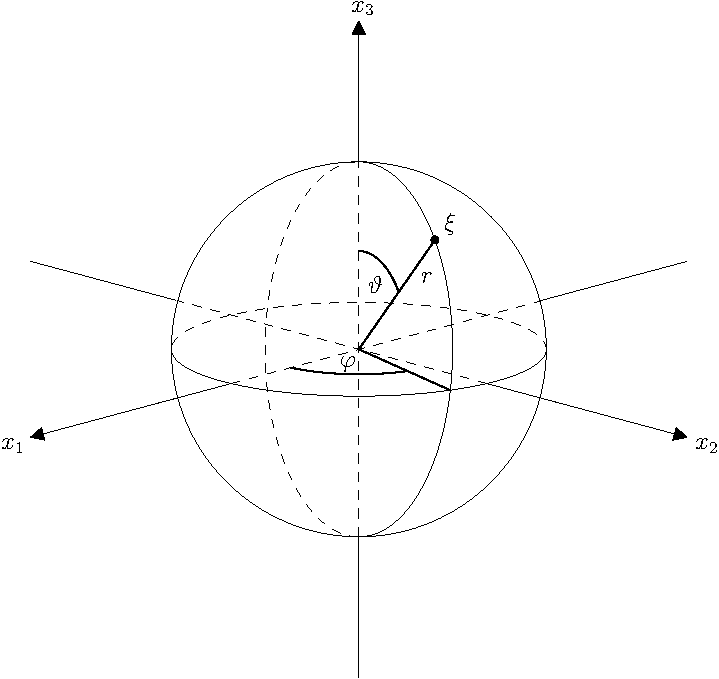
\includegraphics[width=0.45\textwidth]{sphere}}
 For consistency with the other modules and the conventions used there, we also use {\em swapped\/} {\em scaled\/} {\em spherical\/} {\em coordinates\/} $x_1 := \frac{\varphi}{2\pi}$, $x_2 := \frac{\vartheta}{2\pi}$ and identify a point from $\mathbb{S}^2$ with the vector $\mathbf{x} := \left(x_1,x_2\right) \in [-\frac{1}{2}, \frac{1}{2}) \times [0,\frac{1}{2}]$.\hypertarget{group__nfsft_lp}{}\subsubsection{Legendre Polynomials}\label{group__nfsft_lp}
The {\em Legendre\/} {\em polynomials\/} $P_k : [-1,1] \rightarrow \mathbb{R}$, $k \in \mathbb{N}_{0}$ as {\em classical\/} {\em orthogonal\/} {\em polynomials\/} are given by their corresponding {\em Rodrigues\/} {\em formula\/} \[ P_k(t) := \frac{1}{2^k k!} \frac{\text{d}^k}{\text{d} t^k} \left(t^2-1\right)^k. \] The corresponding three-term recurrence relation is \[ (k+1)P_{k+1}(t) = (2k+1) x P_{k}(t) - k P_{k-1}(t) \quad (k \in \mathbb{N}_0). \] With \[ \left< f,g \right>_{\text{L}^2\left([-1,1]\right)} := \int_{-1}^{1} f(t) g(t) \text{d} t \] being the usual $\text{L}^2\left([-1,1]\right)$ inner product, the Legendre polynomials obey the orthogonality condition \[ \left< P_k,P_l \right>_{\text{L}^2\left([-1,1]\right)} = \frac{2}{2k+1} \delta_{k,l}. \]

\begin{Desc}
\item[Remarks:]The normalisation constant $ c_k := \sqrt{\frac{2k+1}{2}}$ renders the scaled Legendre polynomials $c_k P_k$ orthonormal with respect to the induced $\text{L}^2\left([-1,1]\right)$ norm \[ \|f\|_{\text{L}^2\left([-1,1]\right)} := \left(<f,f>_{\text{L}^2\left([-1,1]\right)}\right)^{1/2} = \left(\int_{-1}^{1} |f(t)|^2 \; \text{d} t\right)^{1/2}. \]\end{Desc}
\hypertarget{group__nfsft_alf}{}\subsubsection{Associated Legendre Functions}\label{group__nfsft_alf}
The {\em associated\/} {\em Legendre\/} {\em functions\/} $P_k^n : [-1,1] \rightarrow \mathbb{R} $, $n \in \mathbb{N}_0$, $k \ge n$ are defined by \[ P_k^n(t) := \left(\frac{(k-n)!}{(k+n)!}\right)^{1/2} \left(1-t^2\right)^{n/2} \frac{\text{d}^n}{\text{d} t^n} P_k(t). \] For $n = 0$, they coincide with the Legendre polynomials, i.e. $P_k^0 = P_k$. The associated Legendre functions obey the three-term recurrence relation \[ P_{k+1}^n(t) = v_{k}^n t P_k^n(t) + w_{k}^n P_{k-1}^n(t) \quad (k \ge n), \] with $P_{n-1}^n(t) := 0$, $P_{n}^n(t) := \frac{\sqrt{(2n)!}}{2^n n!} \left(1-t^2\right)^{n/2}$, and \[ v_{k}^n := \frac{2k+1}{((k-n+1)(k+n+1))^{1/2}}\; ,\qquad w_{k}^n := - \frac{((k-n)(k+n))^{1/2}}{((k-n+1)(k+n+1))^{1/2}}. \] For fixed $n$, the set $\left\{P_k^n:\: k \ge n\right\}$ forms a complete set of orthogonal functions in $\text{L}^2\left([-1,1]\right)$ with \[ \left< P_k^n,P_l^n \right>_{\text{L}^2\left([-1,1]\right)} = \frac{2}{2k+1} \delta_{k,l} \quad (0 \le n \le k,l). \]

\begin{Desc}
\item[Remarks:]The normalisation constant $ c_k = \sqrt{\frac{2k+1}{2}}$ renders the scaled associated Legendre functions $c_k P_k^n$ orthonormal with respect to the induced $\text{L}^2\left([-1,1]\right)$ norm \[ \|f\|_{\text{L}^2\left([-1,1]\right)} := \left(<f,f>_{\text{L}^2\left([-1,1]\right)}\right)^{1/2} = \left(\int_{-1}^{1} |f(t)|^2 \; \text{d} t\right)^{1/2}. \]\end{Desc}
\hypertarget{group__nfsft_sh}{}\subsubsection{Spherical Harmonics}\label{group__nfsft_sh}
The standard orthogonal basis of spherical harmonics for $\text{L}^2 \left(\mathbb{S}^2\right)$ with yet unnormalised basis functions $\tilde{Y}_k^n : \mathbb{S}^2 \rightarrow \mathbb{C}$ is given by \[ \tilde{Y}_k^n(\vartheta,\varphi) := P_k^{|n|}(\cos\vartheta) \mathrm{e}^{\mathrm{i} n \varphi} \] with the usual $\text{L}^2\left(\mathbb{S}^2\right)$ inner product \[ \left< f,g \right>_{\mathrm{L}^2\left(\mathbb{S}^2\right)} := \int_{\mathbb{S}^2} f(\vartheta,\varphi) \overline{g(\vartheta,\varphi)} \: \mathrm{d} \mathbf{\xi} := \int_{-\pi}^{\pi} \int_{0}^{\pi} f(\vartheta,\varphi) \overline{g(\vartheta,\varphi)} \sin \vartheta \; \mathrm{d} \vartheta \; \mathrm{d} \varphi. \] The normalisation constant $c_k^n := \sqrt{\frac{2k+1}{4\pi}}$ renders the scaled basis functions \[ Y_k^n(\vartheta,\varphi) := c_k^n P_k^{|n|}(\cos\vartheta) \mathrm{e}^{\mathrm{i} n \varphi} \] orthonormal with respect to the induced $\text{L}^2\left(\mathbb{S}^2 \right)$ norm \[ \|f\|_{\text{L}^2\left(\mathbb{S}^2\right)} = \left(<f,f>_{\text{L}^2\left(\mathbb{S}^2\right)}\right)^{1/2} = \left(\int_{-\pi}^{\pi} \int_{0}^{\pi} |f(\vartheta,\varphi)|^2 \sin \vartheta \; \mathrm{d} \vartheta \; \mathrm{d} \varphi\right)^{1/2}. \] A function $f \in \mathrm{L}^2\left(\mathbb{S}^2\right)$ has the orthogonal expansion \[ f = \sum_{k=0}^{\infty} \sum_{n=-k}^{k} \hat{f}(k,n) Y_k^n, \] where the coefficients $\hat{f}(k,n) := \left< f, Y_k^{n} \right>_{\mathrm{L}^2\left(\mathbb{S}^2\right)}$ are the {\em spherical\/} {\em Fourier\/} {\em coefficients\/} and the equivalence is understood in the $\mathrm{L}^2$-sense.\hypertarget{group__nfsft_nfsfts}{}\subsection{Nonuniform Fast Spherical Fourier Transforms}\label{group__nfsft_nfsfts}
This section describes the input and output relation of the spherical Fourier transform algorithms and the layout of the corresponding plan structure.\hypertarget{group__nfsft_ndsft}{}\subsubsection{Nonuniform Discrete Spherical Fourier Transform}\label{group__nfsft_ndsft}
The {\em nonuniform\/} {\em discrete\/} {\em spherical\/} {\em Fourier\/} {\em transform\/} ({\em NDSFT\/}) is defined as follows: \[ \begin{array}{rcl} \text{\textbf{Input}} & : & \text{coefficients } \hat{f}(k,n) \in \mathbb{C} \text{ for } k=0,\ldots,N,\;n=-k, \ldots,k,\; N \in \mathbb{N}_0,\\[1ex] & & \text{arbitrary nodes } \mathbf{x}(m) \in [-\frac{1}{2},\frac{1}{2}] \times [0,\frac{1}{2}] \text{ for } m=0,\ldots,M-1, M \in \mathbb{N}. \\[1ex] \text{\textbf{Task}} & : & \text{evaluate } f(m) := f\left( \mathbf{x}(m)\right) = \sum_{k=0}^N \sum_{n=-k}^k \hat{f}_k^n Y_k^n\left(\mathbf{x}(m)\right) \text{ for } m=0,\ldots,M-1. \\[1ex] \text{\textbf{Output}} & : & \text{coefficients } f(m) \in \mathbb{C} \text{ for } m=0,\ldots,M-1.\\ \end{array} \]\hypertarget{group__nfsft_andsft}{}\subsubsection{Adjoint Nonuniform Discrete Spherical Fourier Transform}\label{group__nfsft_andsft}
The {\em adjoint\/} {\em nonuniform\/} {\em discrete\/} {\em spherical\/} {\em Fourier\/} {\em transform\/} ({\em adjoint\/} {\em NDSFT\/}) is defined as follows: \[ \begin{array}{rcl} \text{\textbf{Input}} & : & \text{coefficients } f(m) \in \mathbb{C} \text{ for } m=0,\ldots,M-1, M \in \mathbb{N},\\ & & \text{arbitrary nodes } \mathbf{x}(m) \in [-\frac{1}{2},\frac{1}{2}] \times [0,\frac{1}{2}] \text{ for } m=0,\ldots,M-1, N \in \mathbb{N}_0.\\[1ex] \text{\textbf{Task}} & : & \text{evaluate } \hat{f}(k,n) := \sum_{m=0}^{M-1} f(m) \overline{Y_k^n\left(\mathbf{x}(m)\right)}cd Do \text{ for } k=0,\ldots,N,\;n=-k,\ldots,k.\\[1ex] \text{\textbf{Output}} & : & \text{coefficients } \hat{f}(k,n) \in \mathbb{C} \text{ for } k=0,\ldots,N,\;n=-k,\ldots,k.\\[1ex] \end{array} \]\hypertarget{group__nfsft_dl}{}\subsubsection{Data Layout}\label{group__nfsft_dl}
This section describes the public layout of the \hyperlink{structnfsft__plan}{nfsft\_\-plan} structure which contains all data for the computation of the aforementioned spherical Fourier transforms. The structure contains private (no read or write allowed), public read-only (only read access permitted), and public read-write (read and write access allowed) members. In the following, we indicate read and write access by {\tt read} and {\tt write}. The public members are structured as follows: \begin{itemize}
\item {\tt N\_\-total} ({\tt read}) The total number of components in {\tt f\_\-hat}. If the bandwidth is $N \in \mathbb{N}_0$, the total number of components in {\tt f\_\-hat} is {\tt N\_\-total} $ = (2N+2)^2$. \item {\tt M\_\-total} ({\tt read}) the total number of samples $M$ \item {\tt f\_\-hat} ({\tt read-write}) The flattened array of spherical Fourier coefficents. The array has length $(2N+2)^2$ such that valid indices $i \in \mathbb{N}_0$ for array access {\tt f\_\-hat} {\tt }\mbox{[} $i$ {\tt }\mbox{]} are $i=0,1,\ldots,(2N+2)^2-1$. However, only read and write access to indices corresponding to spherical Fourier coefficients $\hat{f}(k,n)$ is defined. The index $i$ corresponding to the spherical Fourier coefficient $\hat{f}(k,n)$ with $0 \le k \le M$, $-k \le n \le k$ is $i = (N+2)(N-n+1)+N+k+1$. For convenience, the helper macro \hyperlink{group__nfsft_ga40}{NFSFT\_\-INDEX(k,n)} provides the necessary index calculations such that one can write {\tt f\_\-hat}\mbox{[} {\tt NFSFT\_\-INDEX}($k,n${\tt })\mbox{]} {\tt =} {\tt }... to access the component corresponding to $\hat{f}(k,n)$. The data layout is due to implementation details. \item {\tt f} ({\tt read-write}) the array of coefficients $f(m)$ for $m=0,\ldots,M-1$ such that {\tt f}\mbox{[}$m${\tt }\mbox{]} = $f(m)$ \item {\tt N} ({\tt read}) the bandwidth $N \in \mathbb{N}_0$ \item {\tt x} the array of nodes $\mathbf{x}(m) \in [-\frac{1}{2},\frac{1}{2}] \times [0,\frac{1}{2}]$ for $m = 0, \ldots,M-1$ such that {\tt f}\mbox{[}$2m${\tt }\mbox{]} = $x_1$ and {\tt f}\mbox{[}$2m+1${\tt }\mbox{]} = $x_2$\end{itemize}
\hypertarget{group__nfsft_gtn}{}\subsubsection{Good to know...}\label{group__nfsft_gtn}
When using the routines of this module you should bear in mind the following: \begin{itemize}
\item The bandwidth $N_{\text{max}}$ up to which precomputation is performed is always chosen as the next power of two with respect to the specified maximum bandwidth. \item By default, the NDSFT transforms (see \hyperlink{group__nfsft_ga6}{ndsft\_\-trafo}, \hyperlink{group__nfsft_ga8}{nfsft\_\-trafo}) are allowed to destroy the input {\tt f\_\-hat} while the input {\tt x} is preserved. On the contrary, the adjoint NDSFT transforms (see \hyperlink{group__nfsft_ga7}{ndsft\_\-adjoint}, \hyperlink{group__nfsft_ga9}{nfsft\_\-adjoint}) do not destroy the input {\tt f} and {\tt x} by default. The desired behaviour can be assured by using the \hyperlink{group__nfsft_ga31}{NFSFT\_\-PRESERVE\_\-F\_\-HAT}, \hyperlink{group__nfsft_ga32}{NFSFT\_\-PRESERVE\_\-X}, \hyperlink{group__nfsft_ga33}{NFSFT\_\-PRESERVE\_\-F} and \hyperlink{group__nfsft_ga34}{NFSFT\_\-DESTROY\_\-F\_\-HAT}, \hyperlink{group__nfsft_ga35}{NFSFT\_\-DESTROY\_\-X}, \hyperlink{group__nfsft_ga36}{NFSFT\_\-DESTROY\_\-F} flags. \end{itemize}


\subsection{Define Documentation}
\hypertarget{group__nfsft_ga25}{
\index{nfsft@{nfsft}!NFSFT_NORMALIZED@{NFSFT\_\-NORMALIZED}}
\index{NFSFT_NORMALIZED@{NFSFT\_\-NORMALIZED}!nfsft@{nfsft}}
\subsubsection[NFSFT\_\-NORMALIZED]{\setlength{\rightskip}{0pt plus 5cm}\#define NFSFT\_\-NORMALIZED~(1U $<$$<$ 0)}}
\label{group__nfsft_ga25}


By default, all computations are performed with respect to the unnormalized basis functions \[ \tilde{Y}_k^n(\vartheta,\varphi) = P_k^{|n|}(\cos\vartheta) \mathrm{e}^{\mathrm{i} n \varphi}. \] If this flag is set, all computations are carried out using the $L_2$- normalized basis functions \[ Y_k^n(\vartheta,\varphi) = \sqrt{\frac{2k+1}{4\pi}} P_k^{|n|}(\cos\vartheta) \mathrm{e}^{\mathrm{i} n \varphi}. \]. 

\begin{Desc}
\item[See also:]\hyperlink{group__nfsft_ga1}{nfsft\_\-init} 

\hyperlink{group__nfsft_ga2}{nfsft\_\-init\_\-advanced} 

\hyperlink{group__nfsft_ga3}{nfsft\_\-init\_\-guru} \end{Desc}
\begin{Desc}
\item[Author:]Jens Keiner \end{Desc}


Definition at line 1718 of file nfft3.h.

Referenced by main(), ndsft\_\-adjoint(), ndsft\_\-trafo(), nfsft\_\-adjoint(), and nfsft\_\-trafo().\hypertarget{group__nfsft_ga26}{
\index{nfsft@{nfsft}!NFSFT_USE_NDFT@{NFSFT\_\-USE\_\-NDFT}}
\index{NFSFT_USE_NDFT@{NFSFT\_\-USE\_\-NDFT}!nfsft@{nfsft}}
\subsubsection[NFSFT\_\-USE\_\-NDFT]{\setlength{\rightskip}{0pt plus 5cm}\#define NFSFT\_\-USE\_\-NDFT~(1U $<$$<$ 1)}}
\label{group__nfsft_ga26}


If this flag is set, the fast NFSFT algorithms (see \hyperlink{group__nfsft_ga8}{nfsft\_\-trafo}, \hyperlink{group__nfsft_ga9}{nfsft\_\-adjoint}) will use internally the exact but usually slower direct NDFT algorithm in favor of fast but approximative NFFT algorithm. 

\begin{Desc}
\item[See also:]\hyperlink{group__nfsft_ga1}{nfsft\_\-init} 

\hyperlink{group__nfsft_ga2}{nfsft\_\-init\_\-advanced} 

\hyperlink{group__nfsft_ga3}{nfsft\_\-init\_\-guru} \end{Desc}
\begin{Desc}
\item[Author:]Jens Keiner \end{Desc}


Definition at line 1730 of file nfft3.h.

Referenced by main(), nfsft\_\-adjoint(), and nfsft\_\-trafo().\hypertarget{group__nfsft_ga27}{
\index{nfsft@{nfsft}!NFSFT_USE_DPT@{NFSFT\_\-USE\_\-DPT}}
\index{NFSFT_USE_DPT@{NFSFT\_\-USE\_\-DPT}!nfsft@{nfsft}}
\subsubsection[NFSFT\_\-USE\_\-DPT]{\setlength{\rightskip}{0pt plus 5cm}\#define NFSFT\_\-USE\_\-DPT~(1U $<$$<$ 2)}}
\label{group__nfsft_ga27}


If this flag is set, the fast NFSFT algorithms (see \hyperlink{group__nfsft_ga8}{nfsft\_\-trafo}, \hyperlink{group__nfsft_ga9}{nfsft\_\-adjoint}) will use internally the usually slower direct DPT algorithm in favor of the fast FPT algorithm. 

\begin{Desc}
\item[See also:]\hyperlink{group__nfsft_ga1}{nfsft\_\-init} 

\hyperlink{group__nfsft_ga2}{nfsft\_\-init\_\-advanced} 

\hyperlink{group__nfsft_ga3}{nfsft\_\-init\_\-guru} \end{Desc}
\begin{Desc}
\item[Author:]Jens Keiner \end{Desc}
\begin{Desc}
\item[Warning:]This feature is not implemented yet! \end{Desc}


Definition at line 1743 of file nfft3.h.

Referenced by main(), nfsft\_\-adjoint(), and nfsft\_\-trafo().\hypertarget{group__nfsft_ga28}{
\index{nfsft@{nfsft}!NFSFT_MALLOC_X@{NFSFT\_\-MALLOC\_\-X}}
\index{NFSFT_MALLOC_X@{NFSFT\_\-MALLOC\_\-X}!nfsft@{nfsft}}
\subsubsection[NFSFT\_\-MALLOC\_\-X]{\setlength{\rightskip}{0pt plus 5cm}\#define NFSFT\_\-MALLOC\_\-X~(1U $<$$<$ 3)}}
\label{group__nfsft_ga28}


If this flag is set, the init methods (see \hyperlink{group__nfsft_ga1}{nfsft\_\-init} , \hyperlink{group__nfsft_ga2}{nfsft\_\-init\_\-advanced} , and \hyperlink{group__nfsft_ga3}{nfsft\_\-init\_\-guru}) will allocate memory and the method \hyperlink{group__nfsft_ga10}{nfsft\_\-finalize} will free the array {\tt x} for you. 

Otherwise, you have to assure by yourself that {\tt x} points to an array of proper size before excuting a transform and you are responsible for freeing the corresponding memory before program termination.

\begin{Desc}
\item[See also:]\hyperlink{group__nfsft_ga1}{nfsft\_\-init} 

\hyperlink{group__nfsft_ga2}{nfsft\_\-init\_\-advanced} 

\hyperlink{group__nfsft_ga3}{nfsft\_\-init\_\-guru} \end{Desc}
\begin{Desc}
\item[Author:]Jens Keiner \end{Desc}


Definition at line 1758 of file nfft3.h.

Referenced by main(), nfsft\_\-finalize(), nfsft\_\-init(), and nfsft\_\-init\_\-guru().\hypertarget{group__nfsft_ga29}{
\index{nfsft@{nfsft}!NFSFT_MALLOC_F_HAT@{NFSFT\_\-MALLOC\_\-F\_\-HAT}}
\index{NFSFT_MALLOC_F_HAT@{NFSFT\_\-MALLOC\_\-F\_\-HAT}!nfsft@{nfsft}}
\subsubsection[NFSFT\_\-MALLOC\_\-F\_\-HAT]{\setlength{\rightskip}{0pt plus 5cm}\#define NFSFT\_\-MALLOC\_\-F\_\-HAT~(1U $<$$<$ 5)}}
\label{group__nfsft_ga29}


If this flag is set, the init methods (see \hyperlink{group__nfsft_ga1}{nfsft\_\-init} , \hyperlink{group__nfsft_ga2}{nfsft\_\-init\_\-advanced} , and \hyperlink{group__nfsft_ga3}{nfsft\_\-init\_\-guru}) will allocate memory and the method \hyperlink{group__nfsft_ga10}{nfsft\_\-finalize} will free the array {\tt f\_\-hat} for you. 

Otherwise, you have to assure by yourself that {\tt f\_\-hat} points to an array of proper size before excuting a transform and you are responsible for freeing the corresponding memory before program termination.

\begin{Desc}
\item[See also:]\hyperlink{group__nfsft_ga1}{nfsft\_\-init} 

\hyperlink{group__nfsft_ga2}{nfsft\_\-init\_\-advanced} 

\hyperlink{group__nfsft_ga3}{nfsft\_\-init\_\-guru} \end{Desc}
\begin{Desc}
\item[Author:]Jens Keiner \end{Desc}


Definition at line 1773 of file nfft3.h.

Referenced by main(), nfsft\_\-finalize(), nfsft\_\-init(), and nfsft\_\-init\_\-guru().\hypertarget{group__nfsft_ga30}{
\index{nfsft@{nfsft}!NFSFT_MALLOC_F@{NFSFT\_\-MALLOC\_\-F}}
\index{NFSFT_MALLOC_F@{NFSFT\_\-MALLOC\_\-F}!nfsft@{nfsft}}
\subsubsection[NFSFT\_\-MALLOC\_\-F]{\setlength{\rightskip}{0pt plus 5cm}\#define NFSFT\_\-MALLOC\_\-F~(1U $<$$<$ 6)}}
\label{group__nfsft_ga30}


If this flag is set, the init methods (see \hyperlink{group__nfsft_ga1}{nfsft\_\-init} , \hyperlink{group__nfsft_ga2}{nfsft\_\-init\_\-advanced} , and \hyperlink{group__nfsft_ga3}{nfsft\_\-init\_\-guru}) will allocate memory and the method \hyperlink{group__nfsft_ga10}{nfsft\_\-finalize} will free the array {\tt f} for you. 

Otherwise, you have to assure by yourself that {\tt f} points to an array of proper size before excuting a transform and you are responsible for freeing the corresponding memory before program termination.

\begin{Desc}
\item[See also:]\hyperlink{group__nfsft_ga1}{nfsft\_\-init} 

\hyperlink{group__nfsft_ga2}{nfsft\_\-init\_\-advanced} 

\hyperlink{group__nfsft_ga3}{nfsft\_\-init\_\-guru} \end{Desc}
\begin{Desc}
\item[Author:]Jens Keiner \end{Desc}


Definition at line 1788 of file nfft3.h.

Referenced by main(), nfsft\_\-finalize(), nfsft\_\-init(), and nfsft\_\-init\_\-guru().\hypertarget{group__nfsft_ga31}{
\index{nfsft@{nfsft}!NFSFT_PRESERVE_F_HAT@{NFSFT\_\-PRESERVE\_\-F\_\-HAT}}
\index{NFSFT_PRESERVE_F_HAT@{NFSFT\_\-PRESERVE\_\-F\_\-HAT}!nfsft@{nfsft}}
\subsubsection[NFSFT\_\-PRESERVE\_\-F\_\-HAT]{\setlength{\rightskip}{0pt plus 5cm}\#define NFSFT\_\-PRESERVE\_\-F\_\-HAT~(1U $<$$<$ 7)}}
\label{group__nfsft_ga31}


If this flag is set, it is guaranteed that during an execution of \hyperlink{group__nfsft_ga6}{ndsft\_\-trafo} or \hyperlink{group__nfsft_ga8}{nfsft\_\-trafo} the content of {\tt f\_\-hat} remains unchanged. 

\begin{Desc}
\item[See also:]\hyperlink{group__nfsft_ga1}{nfsft\_\-init} 

\hyperlink{group__nfsft_ga2}{nfsft\_\-init\_\-advanced} 

\hyperlink{group__nfsft_ga3}{nfsft\_\-init\_\-guru} \end{Desc}
\begin{Desc}
\item[Author:]Jens Keiner \end{Desc}


Definition at line 1800 of file nfft3.h.

Referenced by ndsft\_\-trafo(), nfsft\_\-finalize(), nfsft\_\-init\_\-guru(), and nfsft\_\-trafo().\hypertarget{group__nfsft_ga32}{
\index{nfsft@{nfsft}!NFSFT_PRESERVE_X@{NFSFT\_\-PRESERVE\_\-X}}
\index{NFSFT_PRESERVE_X@{NFSFT\_\-PRESERVE\_\-X}!nfsft@{nfsft}}
\subsubsection[NFSFT\_\-PRESERVE\_\-X]{\setlength{\rightskip}{0pt plus 5cm}\#define NFSFT\_\-PRESERVE\_\-X~(1U $<$$<$ 8)}}
\label{group__nfsft_ga32}


If this flag is set, it is guaranteed that during an execution of \hyperlink{group__nfsft_ga6}{ndsft\_\-trafo}, \hyperlink{group__nfsft_ga8}{nfsft\_\-trafo} or \hyperlink{group__nfsft_ga7}{ndsft\_\-adjoint}, \hyperlink{group__nfsft_ga9}{nfsft\_\-adjoint} the content of {\tt x} remains unchanged. 

\begin{Desc}
\item[See also:]\hyperlink{group__nfsft_ga1}{nfsft\_\-init} 

\hyperlink{group__nfsft_ga2}{nfsft\_\-init\_\-advanced} 

\hyperlink{group__nfsft_ga3}{nfsft\_\-init\_\-guru} \end{Desc}
\begin{Desc}
\item[Author:]Jens Keiner \end{Desc}


Definition at line 1813 of file nfft3.h.\hypertarget{group__nfsft_ga33}{
\index{nfsft@{nfsft}!NFSFT_PRESERVE_F@{NFSFT\_\-PRESERVE\_\-F}}
\index{NFSFT_PRESERVE_F@{NFSFT\_\-PRESERVE\_\-F}!nfsft@{nfsft}}
\subsubsection[NFSFT\_\-PRESERVE\_\-F]{\setlength{\rightskip}{0pt plus 5cm}\#define NFSFT\_\-PRESERVE\_\-F~(1U $<$$<$ 9)}}
\label{group__nfsft_ga33}


If this flag is set, it is guaranteed that during an execution of \hyperlink{group__nfsft_ga7}{ndsft\_\-adjoint} or \hyperlink{group__nfsft_ga9}{nfsft\_\-adjoint} the content of {\tt f} remains unchanged. 

\begin{Desc}
\item[See also:]\hyperlink{group__nfsft_ga1}{nfsft\_\-init} 

\hyperlink{group__nfsft_ga2}{nfsft\_\-init\_\-advanced} 

\hyperlink{group__nfsft_ga3}{nfsft\_\-init\_\-guru} \end{Desc}
\begin{Desc}
\item[Author:]Jens Keiner \end{Desc}


Definition at line 1825 of file nfft3.h.\hypertarget{group__nfsft_ga34}{
\index{nfsft@{nfsft}!NFSFT_DESTROY_F_HAT@{NFSFT\_\-DESTROY\_\-F\_\-HAT}}
\index{NFSFT_DESTROY_F_HAT@{NFSFT\_\-DESTROY\_\-F\_\-HAT}!nfsft@{nfsft}}
\subsubsection[NFSFT\_\-DESTROY\_\-F\_\-HAT]{\setlength{\rightskip}{0pt plus 5cm}\#define NFSFT\_\-DESTROY\_\-F\_\-HAT~(1U $<$$<$ 10)}}
\label{group__nfsft_ga34}


If this flag is set, it is explicitely allowed that during an execution of \hyperlink{group__nfsft_ga6}{ndsft\_\-trafo} or \hyperlink{group__nfsft_ga8}{nfsft\_\-trafo} the content of {\tt f\_\-hat} may be changed. 

\begin{Desc}
\item[See also:]\hyperlink{group__nfsft_ga1}{nfsft\_\-init} 

\hyperlink{group__nfsft_ga2}{nfsft\_\-init\_\-advanced} 

\hyperlink{group__nfsft_ga3}{nfsft\_\-init\_\-guru} \end{Desc}
\begin{Desc}
\item[Author:]Jens Keiner \end{Desc}


Definition at line 1836 of file nfft3.h.\hypertarget{group__nfsft_ga35}{
\index{nfsft@{nfsft}!NFSFT_DESTROY_X@{NFSFT\_\-DESTROY\_\-X}}
\index{NFSFT_DESTROY_X@{NFSFT\_\-DESTROY\_\-X}!nfsft@{nfsft}}
\subsubsection[NFSFT\_\-DESTROY\_\-X]{\setlength{\rightskip}{0pt plus 5cm}\#define NFSFT\_\-DESTROY\_\-X~(1U $<$$<$ 11)}}
\label{group__nfsft_ga35}


If this flag is set, it is explicitely allowed that during an execution of \hyperlink{group__nfsft_ga6}{ndsft\_\-trafo}, \hyperlink{group__nfsft_ga8}{nfsft\_\-trafo} or \hyperlink{group__nfsft_ga7}{ndsft\_\-adjoint}, \hyperlink{group__nfsft_ga9}{nfsft\_\-adjoint} the content of {\tt x} may be changed. 

\begin{Desc}
\item[See also:]\hyperlink{group__nfsft_ga1}{nfsft\_\-init} 

\hyperlink{group__nfsft_ga2}{nfsft\_\-init\_\-advanced} 

\hyperlink{group__nfsft_ga3}{nfsft\_\-init\_\-guru} \end{Desc}
\begin{Desc}
\item[Author:]Jens Keiner \end{Desc}


Definition at line 1848 of file nfft3.h.\hypertarget{group__nfsft_ga36}{
\index{nfsft@{nfsft}!NFSFT_DESTROY_F@{NFSFT\_\-DESTROY\_\-F}}
\index{NFSFT_DESTROY_F@{NFSFT\_\-DESTROY\_\-F}!nfsft@{nfsft}}
\subsubsection[NFSFT\_\-DESTROY\_\-F]{\setlength{\rightskip}{0pt plus 5cm}\#define NFSFT\_\-DESTROY\_\-F~(1U $<$$<$ 12)}}
\label{group__nfsft_ga36}


If this flag is set, it is explicitely allowed that during an execution of \hyperlink{group__nfsft_ga7}{ndsft\_\-adjoint} or \hyperlink{group__nfsft_ga9}{nfsft\_\-adjoint} the content of {\tt f} may be changed. 

\begin{Desc}
\item[See also:]\hyperlink{group__nfsft_ga1}{nfsft\_\-init} 

\hyperlink{group__nfsft_ga2}{nfsft\_\-init\_\-advanced} 

\hyperlink{group__nfsft_ga3}{nfsft\_\-init\_\-guru} \end{Desc}
\begin{Desc}
\item[Author:]Jens Keiner \end{Desc}


Definition at line 1859 of file nfft3.h.\hypertarget{group__nfsft_ga37}{
\index{nfsft@{nfsft}!NFSFT_NO_DIRECT_ALGORITHM@{NFSFT\_\-NO\_\-DIRECT\_\-ALGORITHM}}
\index{NFSFT_NO_DIRECT_ALGORITHM@{NFSFT\_\-NO\_\-DIRECT\_\-ALGORITHM}!nfsft@{nfsft}}
\subsubsection[NFSFT\_\-NO\_\-DIRECT\_\-ALGORITHM]{\setlength{\rightskip}{0pt plus 5cm}\#define NFSFT\_\-NO\_\-DIRECT\_\-ALGORITHM~(1U $<$$<$ 13)}}
\label{group__nfsft_ga37}


If this flag is set, the transforms \hyperlink{group__nfsft_ga6}{ndsft\_\-trafo} and \hyperlink{group__nfsft_ga7}{ndsft\_\-adjoint} do not work. 

Setting this flag saves some memory for precomputed data.

\begin{Desc}
\item[See also:]\hyperlink{group__nfsft_ga4}{nfsft\_\-precompute} 

\hyperlink{group__nfsft_ga6}{ndsft\_\-trafo} 

\hyperlink{group__nfsft_ga7}{ndsft\_\-adjoint} \end{Desc}
\begin{Desc}
\item[Author:]Jens Keiner \end{Desc}


Definition at line 1872 of file nfft3.h.

Referenced by ndsft\_\-adjoint(), ndsft\_\-trafo(), nfsft\_\-forget(), and nfsft\_\-precompute().\hypertarget{group__nfsft_ga38}{
\index{nfsft@{nfsft}!NFSFT_NO_FAST_ALGORITHM@{NFSFT\_\-NO\_\-FAST\_\-ALGORITHM}}
\index{NFSFT_NO_FAST_ALGORITHM@{NFSFT\_\-NO\_\-FAST\_\-ALGORITHM}!nfsft@{nfsft}}
\subsubsection[NFSFT\_\-NO\_\-FAST\_\-ALGORITHM]{\setlength{\rightskip}{0pt plus 5cm}\#define NFSFT\_\-NO\_\-FAST\_\-ALGORITHM~(1U $<$$<$ 14)}}
\label{group__nfsft_ga38}


If this flag is set, the transforms \hyperlink{group__nfsft_ga8}{nfsft\_\-trafo} and \hyperlink{group__nfsft_ga9}{nfsft\_\-adjoint} do not work. 

Setting this flag saves memory for precomputed data.

\begin{Desc}
\item[See also:]\hyperlink{group__nfsft_ga4}{nfsft\_\-precompute} 

\hyperlink{group__nfsft_ga8}{nfsft\_\-trafo} 

\hyperlink{group__nfsft_ga9}{nfsft\_\-adjoint} \end{Desc}
\begin{Desc}
\item[Author:]Jens Keiner \end{Desc}


Definition at line 1883 of file nfft3.h.

Referenced by main(), nfsft\_\-adjoint(), nfsft\_\-forget(), nfsft\_\-init\_\-guru(), nfsft\_\-precompute(), and nfsft\_\-trafo().\hypertarget{group__nfsft_ga39}{
\index{nfsft@{nfsft}!NFSFT_ZERO_F_HAT@{NFSFT\_\-ZERO\_\-F\_\-HAT}}
\index{NFSFT_ZERO_F_HAT@{NFSFT\_\-ZERO\_\-F\_\-HAT}!nfsft@{nfsft}}
\subsubsection[NFSFT\_\-ZERO\_\-F\_\-HAT]{\setlength{\rightskip}{0pt plus 5cm}\#define NFSFT\_\-ZERO\_\-F\_\-HAT~(1U $<$$<$ 16)}}
\label{group__nfsft_ga39}


If this flag is set, the transforms \hyperlink{group__nfsft_ga9}{nfsft\_\-adjoint} and \hyperlink{group__nfsft_ga7}{ndsft\_\-adjoint} set all unused entries in {\tt f\_\-hat} not corresponding to spherical Fourier coefficients to zero. 

\begin{Desc}
\item[Author:]Jens Keiner \end{Desc}


Definition at line 1892 of file nfft3.h.

Referenced by main(), ndsft\_\-adjoint(), and nfsft\_\-adjoint().\hypertarget{group__nfsft_ga46}{
\index{nfsft@{nfsft}!NFSFT_DEFAULT_NFFT_CUTOFF@{NFSFT\_\-DEFAULT\_\-NFFT\_\-CUTOFF}}
\index{NFSFT_DEFAULT_NFFT_CUTOFF@{NFSFT\_\-DEFAULT\_\-NFFT\_\-CUTOFF}!nfsft@{nfsft}}
\subsubsection[NFSFT\_\-DEFAULT\_\-NFFT\_\-CUTOFF]{\setlength{\rightskip}{0pt plus 5cm}\#define NFSFT\_\-DEFAULT\_\-NFFT\_\-CUTOFF~6}}
\label{group__nfsft_ga46}


The default NFFT cutoff parameter. 

\begin{Desc}
\item[Author:]Jens Keiner \end{Desc}


Definition at line 34 of file nfsft.c.

Referenced by nfsft\_\-init\_\-advanced().\hypertarget{group__nfsft_ga47}{
\index{nfsft@{nfsft}!NFSFT_DEFAULT_THRESHOLD@{NFSFT\_\-DEFAULT\_\-THRESHOLD}}
\index{NFSFT_DEFAULT_THRESHOLD@{NFSFT\_\-DEFAULT\_\-THRESHOLD}!nfsft@{nfsft}}
\subsubsection[NFSFT\_\-DEFAULT\_\-THRESHOLD]{\setlength{\rightskip}{0pt plus 5cm}\#define NFSFT\_\-DEFAULT\_\-THRESHOLD~1000}}
\label{group__nfsft_ga47}


The default threshold for the FPT. 

\begin{Desc}
\item[Author:]Jens Keiner \end{Desc}


Definition at line 41 of file nfsft.c.\hypertarget{group__nfsft_ga48}{
\index{nfsft@{nfsft}!NFSFT_BREAK_EVEN@{NFSFT\_\-BREAK\_\-EVEN}}
\index{NFSFT_BREAK_EVEN@{NFSFT\_\-BREAK\_\-EVEN}!nfsft@{nfsft}}
\subsubsection[NFSFT\_\-BREAK\_\-EVEN]{\setlength{\rightskip}{0pt plus 5cm}\#define NFSFT\_\-BREAK\_\-EVEN~5}}
\label{group__nfsft_ga48}


The break-even bandwidth $N \in \mathbb{N}_0$. 

\begin{Desc}
\item[Author:]Jens Keiner \end{Desc}


Definition at line 48 of file nfsft.c.

Referenced by nfsft\_\-adjoint(), nfsft\_\-forget(), nfsft\_\-precompute(), and nfsft\_\-trafo().

\subsection{Function Documentation}
\hypertarget{group__nfsft_ga1}{
\index{nfsft@{nfsft}!nfsft_init@{nfsft\_\-init}}
\index{nfsft_init@{nfsft\_\-init}!nfsft@{nfsft}}
\subsubsection[nfsft\_\-init]{\setlength{\rightskip}{0pt plus 5cm}void nfsft\_\-init (\hyperlink{structnfsft__plan}{nfsft\_\-plan} $\ast$ {\em plan}, int {\em N}, int {\em M})}}
\label{group__nfsft_ga1}


Creates a transform plan. 

\begin{itemize}
\item plan a pointer to a \hyperlink{structnfsft__plan}{nfsft\_\-plan} structure \item N the bandwidth $N \in \mathbb{N}_0$ \item M the number of nodes $M \in \mathbb{N}$\end{itemize}
\begin{Desc}
\item[Author:]Jens Keiner \end{Desc}


Definition at line 225 of file nfsft.c.

References nfsft\_\-init\_\-advanced(), NFSFT\_\-MALLOC\_\-F, NFSFT\_\-MALLOC\_\-F\_\-HAT, and NFSFT\_\-MALLOC\_\-X.\hypertarget{group__nfsft_ga2}{
\index{nfsft@{nfsft}!nfsft_init_advanced@{nfsft\_\-init\_\-advanced}}
\index{nfsft_init_advanced@{nfsft\_\-init\_\-advanced}!nfsft@{nfsft}}
\subsubsection[nfsft\_\-init\_\-advanced]{\setlength{\rightskip}{0pt plus 5cm}void nfsft\_\-init\_\-advanced (\hyperlink{structnfsft__plan}{nfsft\_\-plan} $\ast$ {\em plan}, int {\em N}, int {\em M}, unsigned int {\em nfsft\_\-flags})}}
\label{group__nfsft_ga2}


Creates a transform plan. 

\begin{itemize}
\item plan a pointer to a 

\footnotesize\begin{verbatim} nfsft_plan \end{verbatim}
\normalsize
 structure \item N the bandwidth $N \in \mathbb{N}_0$ \item M the number of nodes $M \in \mathbb{N}$ \item nfsft\_\-flags the NFSFT flags\end{itemize}
\begin{Desc}
\item[Author:]Jens Keiner \end{Desc}


Definition at line 232 of file nfsft.c.

References FFT\_\-OUT\_\-OF\_\-PLACE, FFTW\_\-INIT, NFSFT\_\-DEFAULT\_\-NFFT\_\-CUTOFF, nfsft\_\-init\_\-guru(), PRE\_\-PHI\_\-HUT, and PRE\_\-PSI.

Referenced by nfsft\_\-init().\hypertarget{group__nfsft_ga3}{
\index{nfsft@{nfsft}!nfsft_init_guru@{nfsft\_\-init\_\-guru}}
\index{nfsft_init_guru@{nfsft\_\-init\_\-guru}!nfsft@{nfsft}}
\subsubsection[nfsft\_\-init\_\-guru]{\setlength{\rightskip}{0pt plus 5cm}void nfsft\_\-init\_\-guru (\hyperlink{structnfsft__plan}{nfsft\_\-plan} $\ast$ {\em plan}, int {\em N}, int {\em M}, unsigned int {\em flags}, int {\em nfft\_\-flags}, int {\em nfft\_\-cutoff})}}
\label{group__nfsft_ga3}


Creates a transform plan. 



Definition at line 240 of file nfsft.c.

References nfsft\_\-wisdom::flags, nfft\_\-init\_\-guru(), NFSFT\_\-MALLOC\_\-F, NFSFT\_\-MALLOC\_\-F\_\-HAT, NFSFT\_\-MALLOC\_\-X, NFSFT\_\-NO\_\-FAST\_\-ALGORITHM, and NFSFT\_\-PRESERVE\_\-F\_\-HAT.

Referenced by main(), and nfsft\_\-init\_\-advanced().\hypertarget{group__nfsft_ga4}{
\index{nfsft@{nfsft}!nfsft_precompute@{nfsft\_\-precompute}}
\index{nfsft_precompute@{nfsft\_\-precompute}!nfsft@{nfsft}}
\subsubsection[nfsft\_\-precompute]{\setlength{\rightskip}{0pt plus 5cm}void nfsft\_\-precompute (int {\em N}, double {\em kappa}, unsigned int {\em nfsft\_\-flags}, unsigned int {\em fpt\_\-flags})}}
\label{group__nfsft_ga4}


Performes precomputation up to the next power of two with respect to a given bandwidth $N \in \mathbb{N}_2$. 



Definition at line 326 of file nfsft.c.

References nfsft\_\-wisdom::alpha, alpha\_\-al\_\-all(), nfsft\_\-wisdom::beta, beta\_\-al\_\-all(), nfsft\_\-wisdom::flags, FPT\_\-AL\_\-SYMMETRY, fpt\_\-init(), FPT\_\-PERSISTENT\_\-DATA, fpt\_\-precompute(), nfsft\_\-wisdom::gamma, gamma\_\-al\_\-all(), nfsft\_\-wisdom::initialized, nfsft\_\-wisdom::N\_\-MAX, nfft\_\-next\_\-power\_\-of\_\-2\_\-exp(), NFSFT\_\-BREAK\_\-EVEN, NFSFT\_\-NO\_\-DIRECT\_\-ALGORITHM, NFSFT\_\-NO\_\-FAST\_\-ALGORITHM, nfsft\_\-wisdom::set, nfsft\_\-wisdom::T\_\-MAX, and wisdom.

Referenced by main().\hypertarget{group__nfsft_ga5}{
\index{nfsft@{nfsft}!nfsft_forget@{nfsft\_\-forget}}
\index{nfsft_forget@{nfsft\_\-forget}!nfsft@{nfsft}}
\subsubsection[nfsft\_\-forget]{\setlength{\rightskip}{0pt plus 5cm}void nfsft\_\-forget ()}}
\label{group__nfsft_ga5}


Forgets all precomputed data. 

\begin{Desc}
\item[Author:]Jens Keiner \end{Desc}


Definition at line 428 of file nfsft.c.

References nfsft\_\-wisdom::alpha, nfsft\_\-wisdom::beta, nfsft\_\-wisdom::flags, fpt\_\-finalize(), nfsft\_\-wisdom::gamma, nfsft\_\-wisdom::initialized, nfsft\_\-wisdom::N\_\-MAX, NFSFT\_\-BREAK\_\-EVEN, NFSFT\_\-NO\_\-DIRECT\_\-ALGORITHM, NFSFT\_\-NO\_\-FAST\_\-ALGORITHM, nfsft\_\-wisdom::set, and wisdom.

Referenced by main().\hypertarget{group__nfsft_ga6}{
\index{nfsft@{nfsft}!ndsft_trafo@{ndsft\_\-trafo}}
\index{ndsft_trafo@{ndsft\_\-trafo}!nfsft@{nfsft}}
\subsubsection[ndsft\_\-trafo]{\setlength{\rightskip}{0pt plus 5cm}void ndsft\_\-trafo (\hyperlink{structnfsft__plan}{nfsft\_\-plan} $\ast$ {\em plan})}}
\label{group__nfsft_ga6}


Executes a direct NDSFT, i.e. 

computes for $m = 0,\ldots,M-1$ \[ f(m) = \sum_{k=0}^N \sum_{n=-k}^k \hat{f}(k,n) Y_k^n\left(2\pi x_1(m), 2\pi x_2(m)\right). \]

\begin{itemize}
\item plan the plan\end{itemize}
\begin{Desc}
\item[Author:]Jens Keiner \end{Desc}


Definition at line 501 of file nfsft.c.

References nfsft\_\-wisdom::alpha, nfsft\_\-wisdom::flags, nfsft\_\-wisdom::gamma, NFSFT\_\-INDEX, NFSFT\_\-NO\_\-DIRECT\_\-ALGORITHM, NFSFT\_\-NORMALIZED, NFSFT\_\-PRESERVE\_\-F\_\-HAT, PI, and wisdom.

Referenced by main(), and nfsft\_\-trafo().\hypertarget{group__nfsft_ga7}{
\index{nfsft@{nfsft}!ndsft_adjoint@{ndsft\_\-adjoint}}
\index{ndsft_adjoint@{ndsft\_\-adjoint}!nfsft@{nfsft}}
\subsubsection[ndsft\_\-adjoint]{\setlength{\rightskip}{0pt plus 5cm}void ndsft\_\-adjoint (\hyperlink{structnfsft__plan}{nfsft\_\-plan} $\ast$ {\em plan})}}
\label{group__nfsft_ga7}


Executes a direct adjoint NDSFT, i.e. 

computes for $k=0,\ldots,N; n=-k,\ldots,k$ \[ \hat{f}(k,n) = \sum_{m = 0}^{M-1} f(m) Y_k^n\left(2\pi x_1(m), 2\pi x_2(m)\right). \]

\begin{itemize}
\item plan the plan\end{itemize}
\begin{Desc}
\item[Author:]Jens Keiner \end{Desc}


Definition at line 633 of file nfsft.c.

References nfsft\_\-wisdom::alpha, nfsft\_\-wisdom::flags, nfsft\_\-wisdom::gamma, NFSFT\_\-INDEX, NFSFT\_\-NO\_\-DIRECT\_\-ALGORITHM, NFSFT\_\-NORMALIZED, NFSFT\_\-ZERO\_\-F\_\-HAT, PI, and wisdom.

Referenced by main(), and nfsft\_\-adjoint().\hypertarget{group__nfsft_ga8}{
\index{nfsft@{nfsft}!nfsft_trafo@{nfsft\_\-trafo}}
\index{nfsft_trafo@{nfsft\_\-trafo}!nfsft@{nfsft}}
\subsubsection[nfsft\_\-trafo]{\setlength{\rightskip}{0pt plus 5cm}void nfsft\_\-trafo (\hyperlink{structnfsft__plan}{nfsft\_\-plan} $\ast$ {\em plan})}}
\label{group__nfsft_ga8}


Executes a NFSFT, i.e. 

computes for $m = 0,\ldots,M-1$ \[ f(m) = \sum_{k=0}^N \sum_{n=-k}^k \hat{f}(k,n) Y_k^n\left(2\pi x_1(m), 2\pi x_2(m)\right). \]

\begin{itemize}
\item plan the plan\end{itemize}
\begin{Desc}
\item[Author:]Jens Keiner \end{Desc}


Definition at line 745 of file nfsft.c.

References c2e(), dpt\_\-trafo(), nfsft\_\-wisdom::flags, fpt\_\-trafo(), nfsft\_\-wisdom::initialized, fpt\_\-set\_\-s\_\-::N, nfsft\_\-wisdom::N\_\-MAX, ndft\_\-trafo(), ndsft\_\-trafo(), nfft\_\-trafo(), NFSFT\_\-BREAK\_\-EVEN, NFSFT\_\-INDEX, NFSFT\_\-NO\_\-FAST\_\-ALGORITHM, NFSFT\_\-NORMALIZED, NFSFT\_\-PRESERVE\_\-F\_\-HAT, NFSFT\_\-USE\_\-DPT, NFSFT\_\-USE\_\-NDFT, PI, nfsft\_\-wisdom::set, and wisdom.

Referenced by main().\hypertarget{group__nfsft_ga9}{
\index{nfsft@{nfsft}!nfsft_adjoint@{nfsft\_\-adjoint}}
\index{nfsft_adjoint@{nfsft\_\-adjoint}!nfsft@{nfsft}}
\subsubsection[nfsft\_\-adjoint]{\setlength{\rightskip}{0pt plus 5cm}void nfsft\_\-adjoint (\hyperlink{structnfsft__plan}{nfsft\_\-plan} $\ast$ {\em plan})}}
\label{group__nfsft_ga9}


Executes an adjoint NFSFT, i.e. 

computes for $k=0,\ldots,N; n=-k,\ldots,k$ \[ \hat{f}(k,n) = \sum_{m = 0}^{M-1} f(m) Y_k^n\left(2\pi x_1(m), 2\pi x_2(m)\right). \]

\begin{itemize}
\item plan the plan\end{itemize}
\begin{Desc}
\item[Author:]Jens Keiner \end{Desc}


Definition at line 864 of file nfsft.c.

References c2e\_\-transposed(), dpt\_\-transposed(), nfsft\_\-wisdom::flags, fpt\_\-transposed(), nfsft\_\-wisdom::initialized, fpt\_\-set\_\-s\_\-::N, nfsft\_\-wisdom::N\_\-MAX, ndft\_\-adjoint(), ndsft\_\-adjoint(), nfft\_\-adjoint(), NFSFT\_\-BREAK\_\-EVEN, NFSFT\_\-INDEX, NFSFT\_\-NO\_\-FAST\_\-ALGORITHM, NFSFT\_\-NORMALIZED, NFSFT\_\-USE\_\-DPT, NFSFT\_\-USE\_\-NDFT, NFSFT\_\-ZERO\_\-F\_\-HAT, PI, nfsft\_\-wisdom::set, and wisdom.

Referenced by main().\hypertarget{group__nfsft_ga10}{
\index{nfsft@{nfsft}!nfsft_finalize@{nfsft\_\-finalize}}
\index{nfsft_finalize@{nfsft\_\-finalize}!nfsft@{nfsft}}
\subsubsection[nfsft\_\-finalize]{\setlength{\rightskip}{0pt plus 5cm}void nfsft\_\-finalize (\hyperlink{structnfsft__plan}{nfsft\_\-plan} $\ast$ {\em plan})}}
\label{group__nfsft_ga10}


Destroys a plan. 

\begin{itemize}
\item plan the plan to be destroyed\end{itemize}
\begin{Desc}
\item[Author:]Jens Keiner \end{Desc}


Definition at line 467 of file nfsft.c.

References nfft\_\-finalize(), NFSFT\_\-MALLOC\_\-F, NFSFT\_\-MALLOC\_\-F\_\-HAT, NFSFT\_\-MALLOC\_\-X, and NFSFT\_\-PRESERVE\_\-F\_\-HAT.

Referenced by main().\hypertarget{group__nfsft_ga12}{
\index{nfsft@{nfsft}!alpha_al@{alpha\_\-al}}
\index{alpha_al@{alpha\_\-al}!nfsft@{nfsft}}
\subsubsection[alpha\_\-al]{\setlength{\rightskip}{0pt plus 5cm}double alpha\_\-al (int {\em k}, int {\em n})\hspace{0.3cm}{\tt  \mbox{[}inline\mbox{]}}}}
\label{group__nfsft_ga12}


Computes three-term recurrence coefficients $\alpha_k^n$ of associated Legendre functions. 

\begin{itemize}
\item k The index $k$ \item n The index $n$ \end{itemize}


Definition at line 9 of file legendre.c.

Referenced by alpha\_\-al\_\-all().\hypertarget{group__nfsft_ga13}{
\index{nfsft@{nfsft}!beta_al@{beta\_\-al}}
\index{beta_al@{beta\_\-al}!nfsft@{nfsft}}
\subsubsection[beta\_\-al]{\setlength{\rightskip}{0pt plus 5cm}double beta\_\-al (int {\em k}, int {\em n})\hspace{0.3cm}{\tt  \mbox{[}inline\mbox{]}}}}
\label{group__nfsft_ga13}


Computes three-term recurrence coefficients $\beta_k^n$ of associated Legendre functions. 

\begin{itemize}
\item k The index $k$ \item n The index $n$ \end{itemize}


Definition at line 36 of file legendre.c.

Referenced by beta\_\-al\_\-all().\hypertarget{group__nfsft_ga14}{
\index{nfsft@{nfsft}!gamma_al@{gamma\_\-al}}
\index{gamma_al@{gamma\_\-al}!nfsft@{nfsft}}
\subsubsection[gamma\_\-al]{\setlength{\rightskip}{0pt plus 5cm}double gamma\_\-al (int {\em k}, int {\em n})\hspace{0.3cm}{\tt  \mbox{[}inline\mbox{]}}}}
\label{group__nfsft_ga14}


Computes three-term recurrence coefficients $\gamma_k^n$ of associated Legendre functions. 

\begin{itemize}
\item k The index $k$ \item n The index $n$ \end{itemize}


Definition at line 48 of file legendre.c.

Referenced by gamma\_\-al\_\-all().\hypertarget{group__nfsft_ga18}{
\index{nfsft@{nfsft}!alpha_al_all@{alpha\_\-al\_\-all}}
\index{alpha_al_all@{alpha\_\-al\_\-all}!nfsft@{nfsft}}
\subsubsection[alpha\_\-al\_\-all]{\setlength{\rightskip}{0pt plus 5cm}void alpha\_\-al\_\-all (double $\ast$ {\em alpha}, int {\em N})\hspace{0.3cm}{\tt  \mbox{[}inline\mbox{]}}}}
\label{group__nfsft_ga18}


Compute three-term-recurrence coefficients $\alpha_{k-1}^n$ of associated Legendre functions for $k,n = 0,1,\ldots,N$. 

\begin{itemize}
\item alpha A pointer to an array of doubles of size $(N+1)^2$ where the coefficients will be stored such that alpha\mbox{[}n+(N+1)+k\mbox{]} = $\alpha_{k-1}^n$. \item N The upper bound $N$. \end{itemize}


Definition at line 106 of file legendre.c.

References alpha\_\-al().

Referenced by nfsft\_\-precompute().\hypertarget{group__nfsft_ga19}{
\index{nfsft@{nfsft}!beta_al_all@{beta\_\-al\_\-all}}
\index{beta_al_all@{beta\_\-al\_\-all}!nfsft@{nfsft}}
\subsubsection[beta\_\-al\_\-all]{\setlength{\rightskip}{0pt plus 5cm}void beta\_\-al\_\-all (double $\ast$ {\em beta}, int {\em N})\hspace{0.3cm}{\tt  \mbox{[}inline\mbox{]}}}}
\label{group__nfsft_ga19}


Compute three-term-recurrence coefficients $\beta_{k-1}^n$ of associated Legendre functions for $k,n = 0,1,\ldots,N$. 

\begin{itemize}
\item beta A pointer to an array of doubles of size $(N+1)^2$ where the coefficients will be stored such that beta\mbox{[}n+(N+1)+k\mbox{]} = $\beta_{k-1}^n$. \item N The upper bound $N$. \end{itemize}


Definition at line 120 of file legendre.c.

References beta\_\-al().

Referenced by nfsft\_\-precompute().\hypertarget{group__nfsft_ga20}{
\index{nfsft@{nfsft}!gamma_al_all@{gamma\_\-al\_\-all}}
\index{gamma_al_all@{gamma\_\-al\_\-all}!nfsft@{nfsft}}
\subsubsection[gamma\_\-al\_\-all]{\setlength{\rightskip}{0pt plus 5cm}void gamma\_\-al\_\-all (double $\ast$ {\em gamma}, int {\em N})\hspace{0.3cm}{\tt  \mbox{[}inline\mbox{]}}}}
\label{group__nfsft_ga20}


Compute three-term-recurrence coefficients $\gamma_{k-1}^n$ of associated Legendre functions for $k,n = 0,1,\ldots,N$. 

\begin{itemize}
\item beta A pointer to an array of doubles of size $(N+1)^2$ where the coefficients will be stored such that gamma\mbox{[}n+(N+1)+k\mbox{]} = $\gamma_{k-1}^n$. \item N The upper bound $N$. \end{itemize}


Definition at line 134 of file legendre.c.

References gamma\_\-al().

Referenced by nfsft\_\-precompute().\hypertarget{group__nfsft_ga21}{
\index{nfsft@{nfsft}!eval_al@{eval\_\-al}}
\index{eval_al@{eval\_\-al}!nfsft@{nfsft}}
\subsubsection[eval\_\-al]{\setlength{\rightskip}{0pt plus 5cm}void eval\_\-al (double $\ast$ {\em x}, double $\ast$ {\em y}, int {\em size}, int {\em k}, double $\ast$ {\em alpha}, double $\ast$ {\em beta}, double $\ast$ {\em gamma})\hspace{0.3cm}{\tt  \mbox{[}inline\mbox{]}}}}
\label{group__nfsft_ga21}


Evaluates an associated Legendre polynomials $P_k^n(x,c)$ using the Clenshaw-algorithm. 

\begin{itemize}
\item x A pointer to an array of nodes where the function is to be evaluated \item y A pointer to an array where the function values are returned \item size The length of x and y \item k The index $k$ \item alpha A pointer to an array containing the recurrence coefficients $\alpha_c^n,\ldots,\alpha_{c+k}^n$ \item beta A pointer to an array containing the recurrence coefficients $\beta_c^n,\ldots,\beta_{c+k}^n$ \item gamma A pointer to an array containing the recurrence coefficients $\gamma_c^n,\ldots,\gamma_{c+k}^n$ \end{itemize}


Definition at line 148 of file legendre.c.\hypertarget{group__nfsft_ga22}{
\index{nfsft@{nfsft}!eval_al_thresh@{eval\_\-al\_\-thresh}}
\index{eval_al_thresh@{eval\_\-al\_\-thresh}!nfsft@{nfsft}}
\subsubsection[eval\_\-al\_\-thresh]{\setlength{\rightskip}{0pt plus 5cm}int eval\_\-al\_\-thresh (double $\ast$ {\em x}, double $\ast$ {\em y}, int {\em size}, int {\em k}, double $\ast$ {\em alpha}, double $\ast$ {\em beta}, double $\ast$ {\em gamma}, double {\em threshold})\hspace{0.3cm}{\tt  \mbox{[}inline\mbox{]}}}}
\label{group__nfsft_ga22}


Evaluates an associated Legendre polynomials $P_k^n(x,c)$ using the Clenshaw-algorithm if it no exceeds a given threshold. 

\begin{itemize}
\item x A pointer to an array of nodes where the function is to be evaluated \item y A pointer to an array where the function values are returned \item size The length of x and y \item k The index $k$ \item alpha A pointer to an array containing the recurrence coefficients $\alpha_c^n,\ldots,\alpha_{c+k}^n$ \item beta A pointer to an array containing the recurrence coefficients $\beta_c^n,\ldots,\beta_{c+k}^n$ \item gamma A pointer to an array containing the recurrence coefficients $\gamma_c^n,\ldots,\gamma_{c+k}^n$ \item threshold The threshold \end{itemize}


Definition at line 193 of file legendre.c.\hypertarget{group__nfsft_ga23}{
\index{nfsft@{nfsft}!c2e@{c2e}}
\index{c2e@{c2e}!nfsft@{nfsft}}
\subsubsection[c2e]{\setlength{\rightskip}{0pt plus 5cm}void c2e (\hyperlink{structnfsft__plan}{nfsft\_\-plan} $\ast$ {\em plan})\hspace{0.3cm}{\tt  \mbox{[}inline\mbox{]}}}}
\label{group__nfsft_ga23}


Converts coefficients $\left(b_k^n\right)_{k=0}^M$ with $M \in \mathbb{N}_0$, $-M \le n \le M$ from a linear combination of Chebyshev polynomials \[ f(\cos\vartheta) = \sum_{k=0}^{2\lfloor\frac{M}{2}\rfloor} a_k (\sin\vartheta)^{n\;\mathrm{mod}\;2} T_k(\cos\vartheta) \] to coefficients $\left(c_k^n\right)_{k=0}^M$ matching the representation by complex exponentials \[ f(\cos\vartheta) = \sum_{k=-M}^{M} c_k \mathrm{e}^{\mathrm{i}k\vartheta} \] for each order $n=-M,\ldots,M$. 

\begin{itemize}
\item plan The {\tt \hyperlink{structnfsft__plan}{nfsft\_\-plan}} containing the coefficients $\left(b_k^n\right)_{k=0,\ldots,M;n=-M,\ldots,M}$\end{itemize}
\begin{Desc}
\item[Remarks:]The transformation is computed in place.\end{Desc}
\begin{Desc}
\item[Author:]Jens Keiner \end{Desc}


Definition at line 80 of file nfsft.c.

References NFSFT\_\-INDEX.

Referenced by nfsft\_\-trafo().\hypertarget{group__nfsft_ga24}{
\index{nfsft@{nfsft}!c2e_transposed@{c2e\_\-transposed}}
\index{c2e_transposed@{c2e\_\-transposed}!nfsft@{nfsft}}
\subsubsection[c2e\_\-transposed]{\setlength{\rightskip}{0pt plus 5cm}void c2e\_\-transposed (\hyperlink{structnfsft__plan}{nfsft\_\-plan} $\ast$ {\em plan})\hspace{0.3cm}{\tt  \mbox{[}inline\mbox{]}}}}
\label{group__nfsft_ga24}


Transposed version of the function \hyperlink{group__nfsft_ga23}{c2e}. 

\begin{itemize}
\item plan The {\tt \hyperlink{structnfsft__plan}{nfsft\_\-plan}} containing the coefficients $\left(c_k^n\right)_{k=-M,\ldots,M;n=-M,\ldots,M}$\end{itemize}
\begin{Desc}
\item[Remarks:]The transformation is computed in place.\end{Desc}
\begin{Desc}
\item[Author:]Jens Keiner \end{Desc}


Definition at line 158 of file nfsft.c.

References NFSFT\_\-INDEX.

Referenced by nfsft\_\-adjoint().

\subsection{Variable Documentation}
\hypertarget{group__nfsft_ga0}{
\index{nfsft@{nfsft}!wisdom@{wisdom}}
\index{wisdom@{wisdom}!nfsft@{nfsft}}
\subsubsection[wisdom]{\setlength{\rightskip}{0pt plus 5cm}struct \hyperlink{structnfsft__wisdom}{nfsft\_\-wisdom} \hyperlink{group__nfsft_ga0}{wisdom} = \{false,0U\}\hspace{0.3cm}{\tt  \mbox{[}static\mbox{]}}}}
\label{group__nfsft_ga0}


The global wisdom structure for precomputed data. 

{\tt wisdom.initialized} is set to {\tt false} and {\tt wisdom.flags} is set to {\tt 0U}.

\begin{Desc}
\item[Author:]Jens Keiner \end{Desc}


Definition at line 56 of file nfsft.c.

Referenced by ndsft\_\-adjoint(), ndsft\_\-trafo(), nfsft\_\-adjoint(), nfsft\_\-forget(), nfsft\_\-precompute(), and nfsft\_\-trafo().